\documentclass[12pt]{beamer}
\usepackage{tikz}
\usepackage[italian]{babel}
\usetheme{Madrid}
\usecolortheme{orchid}

\definecolor{blue}{HTML}{608bf6}
\definecolor{black}{HTML}{1c1c1c}
\definecolor{green}{HTML}{39e600}
\definecolor{grey}{HTML}{949494}

\title{Introduzione alle CTF}
\subtitle{Lezione 1}
\author{Alessandro Righi \and Cristiano Di Bari}
\institute{Università degli Studi di Verona}
\date{3 Novembre 2023}

\begin{document}
\begin{frame}
\titlepage
\end{frame}

\section{Introduzione}

\begin{frame}{Chi siamo?}
\begin{columns}[T] % align columns
\begin{column}{.48\textwidth}
\begin{itemize}
\item laurea magistrale @ UniVR
\item istruttore @ CyberChallenge
\item \textit{System Developer} @ IOTINGA
\end{itemize}        
{\color{blue}\rule{\linewidth}{2pt}}%
\begin{center}
Cristiano Di Bari
\begin{tikzpicture}[inner ysep=0.4cm]
\clip (0,0) circle (1.5cm) node {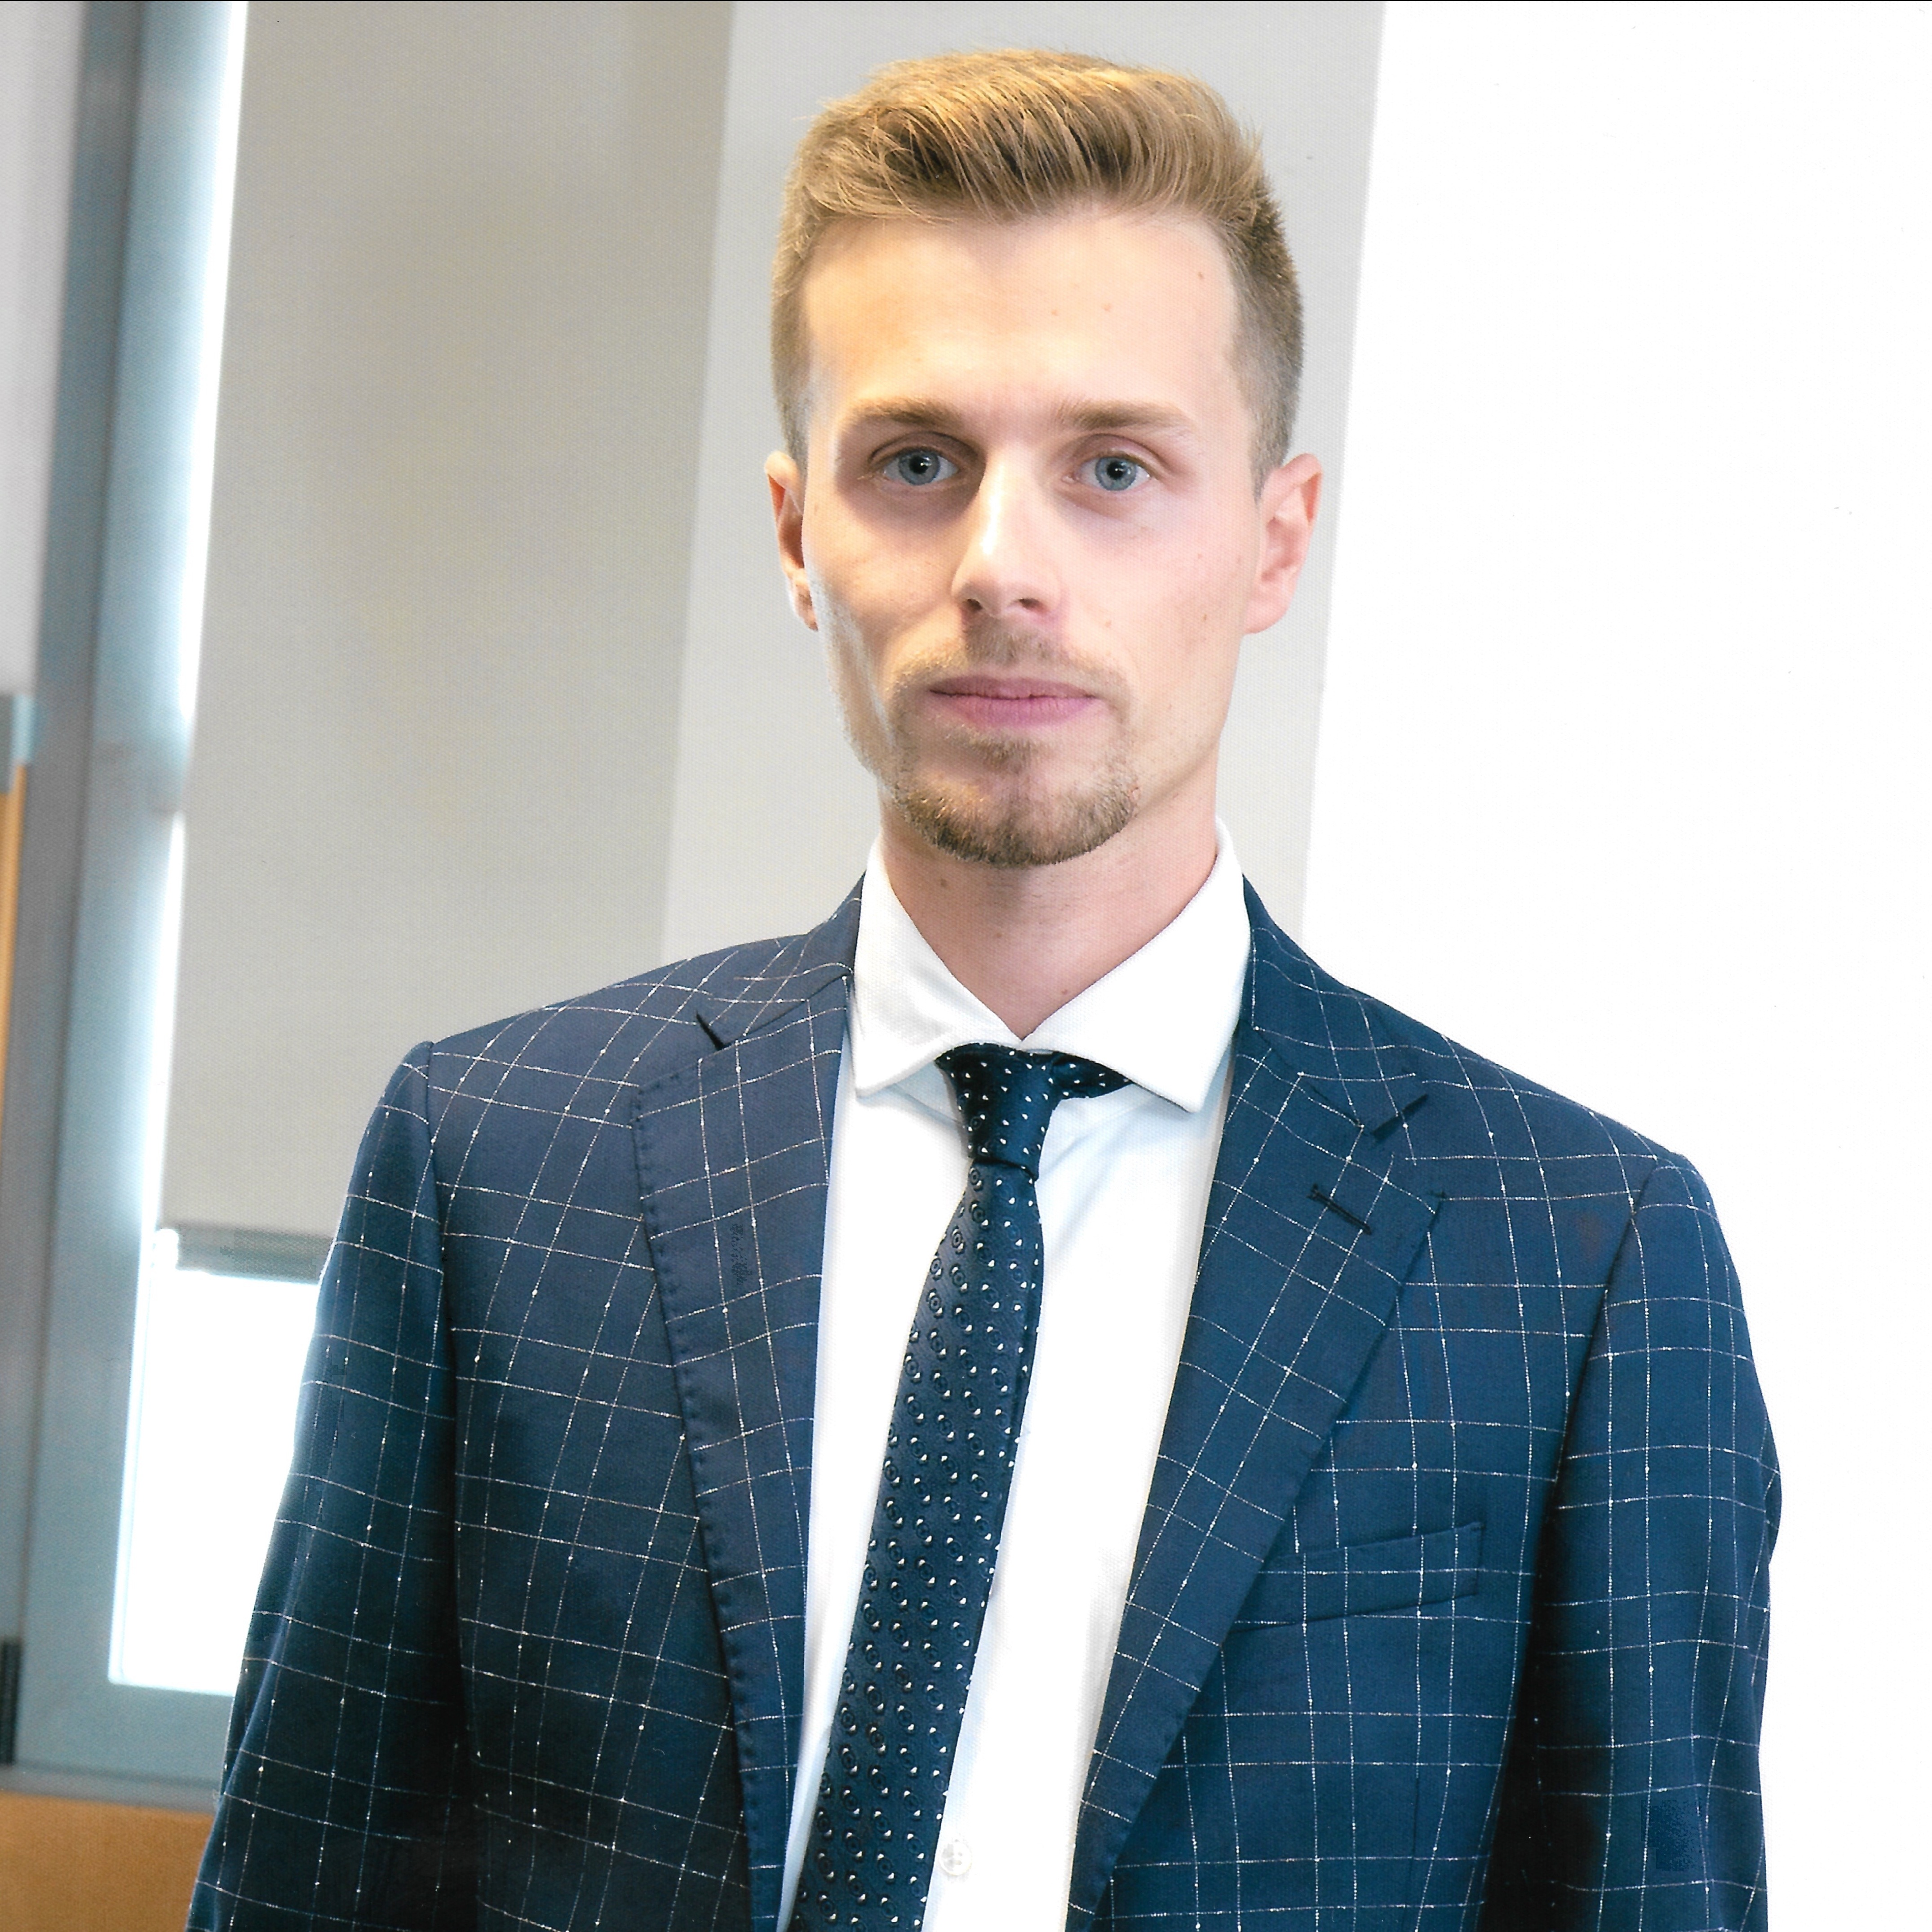
\includegraphics[width=3cm]{img/cris.jpg}};
\end{tikzpicture}
\end{center}
\end{column}%
\hfill%
\begin{column}{.48\textwidth}%
\begin{center}%
\begin{tikzpicture}%
\clip (0,0) circle (1.5cm) node {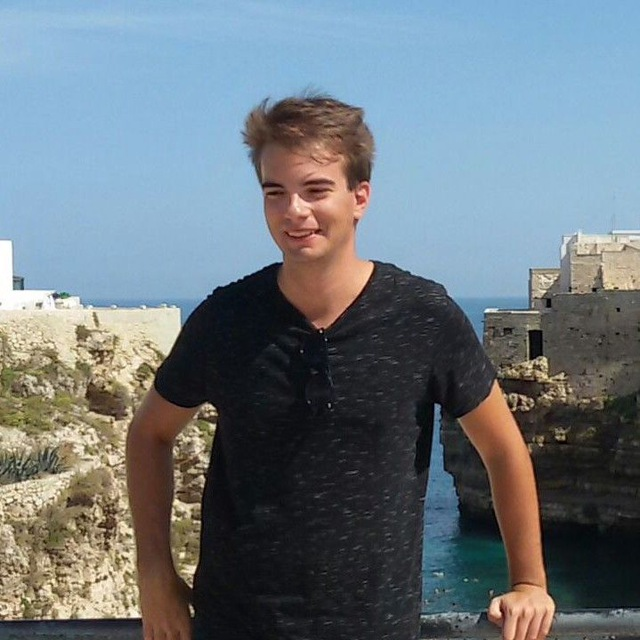
\includegraphics[width=3cm]{img/ale.jpeg}};
\end{tikzpicture}

Alessandro Righi
\color{blue}{\rule{\linewidth}{2pt}}%
\begin{itemize}
\item laurea magistrale @ UniVR
\item istruttore @ CyberChallenge
\item \textit{Applied Research Director} @ IOTINGA
\end{itemize}
\end{center}
\end{column}%
\end{columns}
\end{frame}

\begin{frame}{Cosa sono le CTF?}

Le \textit{Capture The Flag} (CTF) sono delle sfide in cui i partecipanti 
devono trovare delle \textit{flag}, ossia delle stringhe di testo, all'interno
di sistemi informatici contenenti delle vulnerabilità di sicurezza. 
\vfill
\begin{exampleblock}{Esempio di flag}
\texttt{CCIT\{Th1s-1sY0uR-F1rst-Fl4ag\}}
\end{exampleblock}
\vfill
Una volta trovate le flag vanno, solitamente, inviate ad una piattaforma di gara, 
che si occupa di validarle, assegnando il punteggio della challenge nel caso siano corrette.
\end{frame}

\begin{frame}{Perché fare CTF?}
Avete mai fatto CTF?

\pause\vfill

Se no... ecco alcune ragioni per iniziare:
\pause\vfill
\begin{itemize}
\item per divertirsi!
\pause\vfill
\item per imparare cose nuove (tante)
\pause\vfill
\item per scrivere software (più) sicuro
\pause\vfill
\item per conoscere nuova gente, creare networking
\end{itemize}
\end{frame}

\begin{frame}{Tipologie di CTF}
Esistono due tipologie di CTF:
\begin{itemize}
    \item \textit{Jeopardy}: il partecipante attacca una serie di servizi malevoli e sottomette le flag ad un sistema di verifica
    \item \textit{Attack-Defence (AD)}: competizione a squadre dove ogni team deve attaccare i sistemi dell'avversario, e difendere i propri
\end{itemize}

\vfill
Per queste lezioni di concentreremo sul primo tipo (\textit{Jeopardy}), di gran lunga le più diffuse, che è anche
quella organizzata da \textit{Würth Phoenix}.
\end{frame}

\begin{frame}{Tipologie di challenge}
Tipicamente le challenge che si affrontano possono essere di 4 macro categorie:
\begin{itemize}
    \item \textit{Binary}: è necessario ricercare vulnerabilità in un eseguibile, quali ad es. buffer overflow
    \item \textit{Web}: si tratta di trovare vulnerabilità in una web app, web API, o comunque applicativo esposto in rete
    \item \textit{Crypto}: è necessario decodificare un testo cifrato con un algoritmo (ovviamente vulnerabile)
    \item \textit{Misc}: sono challenge che non rientrano in nessuno dei tipi precedenti, e richiedono spesso creatività per essere affrontate
\end{itemize}

Per queste lezioni ci concentreremo sulla categoria \textit{Web}.
\end{frame}

\begin{frame}
\Huge\center Iniziamo!
\end{frame}

\section{Path traversal}
\subsection{Introduzione}
\begin{frame}{Path traversal}

Immaginiamo di avere una pagina web che per caricare l'immagine del profilo di un utente effettua una richiesta a:

\begin{block}{Richiesta}
\texttt{https://mysecureapp.com/assets?name=image.jpeg}
\end{block}

\pause
Cosa succede se modifico la richiesta in questo modo?

\begin{exampleblock}{Richiesta alterata}
\texttt{https://mysecureapp.com/assets?name=../image.jpeg}
\end{exampleblock}
    
\pause

Se il server non effettua adeguati controlli, è possibile leggere file fuori dalla \textit{root} directory del web server!

\end{frame}
\begin{frame}{Path traversal}
Cosa consente di fare questa vulnerabilità?

\pause
\begin{itemize}
    \item leggere \textit{segreti} altrimenti non accessibili, ad es. file di configurazione quali \texttt{/etc/passwd}
    \pause
    \item ottenere il \textit{codice sorgente} dell'applicazione web
    \pause
    \item accedere ai dati di altri utenti, bypassando restrizioni imposte dall'applicazione web
    \pause
\end{itemize}

\begin{alertblock}{Suggerimento}
È possibile aggiungere tanti \texttt{../} fino a raggiungere la directory \textit{root}, ad esempio \texttt{../../../../../etc/passwd}
\end{alertblock}

\end{frame}
\subsection{Challenges}
\begin{frame}{Challenges}
Vediamo la prima challenge. Per queste lezioni utilizzeremo delle challenge 
prese dalla piattaforma di allenamento delle Olimpiadi di Cybersecurity (\url{https://olicyber.it}), 
a cui vi invitiamo ad iscrivevi.
\end{frame}

\begin{frame}{Traverse me}
    % https://training.olicyber.it/challenges#challenge-504
    Ho trovato questa galleria di quadri, chissà se ce ne sono di nascosti.
    \pause
    \begin{itemize}
        \item In questa applicazione vengono caricati dei file salvati sul server, sai individuare dove?
        \pause
        \item Forse è possibile modificare il nome del file per visualizzare altri elementi presenti sul filesystem.
        \pause
    \end{itemize}
    \begin{exampleblock}{Domanda}
        É possibile stampare altri file?
    \end{exampleblock}
\end{frame}

\begin{frame}{Traverse me more}
    % https://training.olicyber.it/challenges#challenge-507
    Questa volta ho fixato il problema della galleria d'arte, non riuscirai mai a carpire il mio segreto.
    \pause
    \begin{itemize}
        \item Provando ad applicare la soluzione per la challenge precedente ci accorgiamo che non funziona!
        \pause
        \item Guardando il codice sorgente, notiamo che viene fatto un \textit{sanitize} del nome del file che rimuove alcuni caratteri.
        \pause
        \item Possiamo bypassare questo controllo?
        \pause
    \end{itemize}
\end{frame}

\begin{frame}{Light or dark}
    % https://training.olicyber.it/challenges#challenge-49
    \begin{itemize}
        \item La challenge mostra un sito web in cui è possibile selezionare il tema, come viene applicato lo stile alla pagina html?
        \pause
        \item Scaricando il file sorgente php notiamo che lo sviluppatore ha applicato dei filtri per evitare che un utente malintenzionato possa caricare un file diverso dai fogli css.
        \pause
        \item Il secondo controllo verifica che l'estensione del file da caricare sia \texttt{.css}, in caso contrario aggiunge l'estensione richiesta tramite una concatenazione di stringhe. Questo controllo sembra difficile da aggirare...o forse no.
        \pause
    \end{itemize}

    \begin{alertblock}{Suggerimento}
        Avete mai sentito parlare di ``Null Byte Injection''?
    \end{alertblock}
\end{frame}


% \subsection{Tool: Burp suite}
\begin{frame}{Flags shop}
% https://training.olicyber.it/challenges#challenge-43
\end{frame}

%%% SQLI 

\section{SQL Injection}
\begin{frame}{}
\end{frame}

\begin{frame}{Basic SQLi}
% https://training.olicyber.it/challenges#challenge-48
\end{frame}

\begin{frame}{Admin's secret}
% https://training.olicyber.it/challenges#challenge-44
\end{frame}

\begin{frame}{Password changer 3000}
    % http://password-changer.challs.olicyber.it
    Riesci a cambiare la password dell'utente "admin"?
    \begin{itemize}
        \item Un sito per cambiare le password degli utenti...non sembra molto utile.
        \pause
        \item Provando a cambiare la password dell'utente ``pippo'' otteniamo in risposta una nuova password. Proviamo ad analizzare la richiesta HTTP che abbiamo appena effettuato. 
        \pause
        \item Dovremmo riuscire ad impersonare l'utente ``admin'', forse la codifica \texttt{Base64} può esserci d'aiuto.
        \pause
    \end{itemize}
\end{frame}

\begin{frame}{Tool: curl}
\end{frame}
\begin{frame}{A TOO small reminder...}
    % https://training.olicyber.it/challenges#challenge-36
\end{frame}

\begin{frame}{ZioFrank}
    % https://training.olicyber.it/challenges#challenge-53
\end{frame}

% \subsection{XSS}

\end{document}
